\chapter{Diagnostics}\label{app:Diagnostics}

The dedicated pedestal experiments, both in I-mode and ELMy H-mode, presented here required an extensive suite of diagnostics to characterize pedestal behavior.  Broadly, these diagnostics may be broken down into three categories:

\begin{description}
 \item[Thomson Scattering] \hfill \\
 Details the edge Thomson scattering diagnostic, from which the high-resolution profile data used for the bulk of this thesis was gathered.
 \item[Fast Diagnostics] \hfill \\
 Details the Electron-Cyclotron Emission (ECE) and $H_\alpha$ line radiation diagnostics used to track sawtooth crashes and ELM events in the plasma edge.
 \item[Fluctuation Diagnostics] \hfill \\
 Details Gas-Puff Imaging (GPI), Reflectometry, and other diagnostics used to characterize the mid-frequency fluctuations found in I-mode pedestals.
\end{description}

\section{Thomson Scattering}\label{sec:app_ts}

Due to the steep gradients in density, temperature, and pressure found in the pedestal, accurate characterization of plasma profiles in this region requires diagnostics capable of very fine spatial resolution.  Measurements based on the Thomson scattering \cite{Sheffield} of laser light off of electrons in the plasma provides the high-resolution pedestal profiles used in this thesis: Thomson scattering is a near-direct measurement of electron temperature and density, independent of bulk plasma parameters (\ie it is unaffected by the cutoffs or reflections found in other diagnostics, and produces no significant perturbation to the plasma).  Measurement via Thomson scattering produces an effective ``snapshot'' of the plasma parameters at each measurement point, with spatial resolution limited only by collection optics geometry, and time resolution limited by repetition rate on the lasers.  Despite significant technical difficulties -- for example, the high-powered lasers and sensitive collection optics needed to capture the weak scattered light and the necessity for careful calibration of density measurements -- Thomson scattering diagnostics remain a versatile and powerful tool for plasma pedestal measurement, and provided the bulk of the profile data used in this thesis.\nicesectionending

\subsection{Principles of Thomson Scattering}\label{subsec:app_background}

An intuitive picture of the Thomson scattering phenomenon may be obtained by the consideration of a stationary, free electron with an EM wave impinging on it.  The particle will be accelerated by the wave (approximately sinusoidally for $E$-field-dominated acceleration at nonrelativistic speeds), causing it to radiate.  Any motion of the electron will cause Doppler shifting in the scattered radiation -- motion relative to the incident wave shifts the incident frequency $\omega_i$, at which the particle oscillates, while motion relative to an observer shifts the scattered wave.  This geometry for general positions of the particle and observer is given in \cref{fig:app_ts_geometry}.

\begin{figure}[t]
 \pushtooutside
 \ffigbox[\FBwidth]{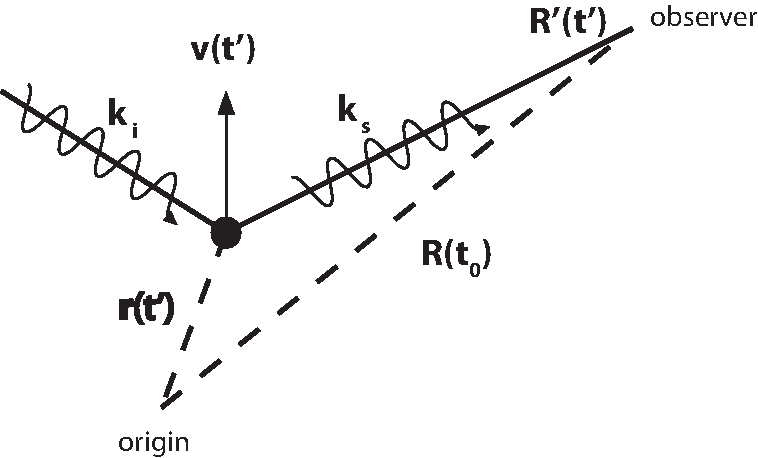
\includegraphics[width=150mm]{graphics/Diagnostics/TS_geometry.pdf}}{\caption{Coordinate system considered for Thomson scattering, with the incident wave of wavenumber $\vec{k}_i$ incident on a particle at $\vec{r}(t')$ for retarded time $t'$.  The scattered wave $\vec{k}_s$ is drawn to an observer at $\vec{R}(t')$.}\label{fig:app_ts_geometry}}
\end{figure}

The scattered electric field from a generally-accelerated electron moving at $\vec{\beta} = \vec{v}/c$ is given from the Lienard-Wiechert potentials \cite[\S 7]{Hutchinson},

\begin{equation}\label{eq:LienardWiechert}
 \begin{gathered}
  \vec{E}_s = \frac{-e}{4\pi\varepsilon_0} \left\llbracket \frac{1}{\kappa^3 Rc} \hat{s} \times \left( \left(\hat{s} \times \vec{\beta}\right) \times \dot{\beta}\right)\right\rrbracket_{t'}\\
  \kappa = 1 = \frac{\vec{R}' \cdot \vec{v}}{R'c} = 1 - \hat{s} \cdot \vec{\beta}, \qquad t' = t - \frac{R'}{c}
  \end{gathered}
\end{equation}

\noindent where $\hat{s}$ indicates the unit vector along the scattering direction, $\vec{R} = R\hat{s}$ is the vector to the observer, $\kappa$ is a relativistic scale factor, and $t'$ is the relativistic retarded time.  The apostrophe indicates a parameter evaluated at the retarded time, \ie $R' = R(t')$; the bracketed term in \cref{eq:LienardWiechert} likewise is evaluated at $t'$.  The scattered power per solid angle is given by

\begin{equation}\label{eq:dPdOmega}
 \begin{aligned}
  \frac{dP_s}{d\Omega} &= R^2 \vec{S}\cdot\hat{s} = R^2 \frac{1}{\mu_0} \left(\vec{E} \times \vec{B}\right)\cdot\hat{s}\\
  &= R^2 \varepsilon_0 c \left(\vec{E}_s \times \left(\hat{s} \times \vec{E}_s\right)\right) \cdot \hat{s} = R^2 c \varepsilon_0 \left|E_s\right|^2
 \end{aligned}
\end{equation}

\noindent Relativistically, the electron motion (which in turn sets the field determined by \cref{eq:LienardWiechert}) is given by

\begin{equation}\label{eq:betadot}
 \dot{\beta} = \frac{d}{dt}\left(\gamma m_e \vec{v}\right) = -e\left(\vec{E}_i + \vec{v} \times \vec{B}_i\right)
\end{equation}

\noindent thus

\begin{equation}\label{eq:betadot2}
 m_e \gamma \dot{\beta} + \gamma^3 m_e \beta \left(\vec{\beta}\cdot\dot{\beta}\right) = -e \left(\frac{\vec{E}_i}{c} + \vec{\beta}\times\vec{B}_i\right)
\end{equation}

\noindent Dotting $\vec{\beta}$ into this and substituting,

\begin{equation}\label{eq:betadot3}
 \dot{\beta} = -\frac{e}{m_e \gamma} \left( \frac{\vec{E}_i}{c} - \frac{\vec{\beta}\cdot\vec{E}_i}{c} \vec{\beta} + \vec{\beta} \times \vec{B}_i \right)
\end{equation}

\noindent The general relativistic solution to \cref{eq:LienardWiechert} with the above is rather intractible, although full relativistic treatments have been done \note{cites, check!}\gnote{cites for relativistic treatment}.  However, the radiated field may be simplified substantially in the nonrelativistic limit -- in the limit of $\beta \ll 1$, the acceleration is simply

\begin{equation}\label{eq:betadot_nonrel}
 \dot{\beta} = -\frac{e}{m_e c}\vec{E}_i
\end{equation}

\noindent and the scattered field is

\begin{equation}\label{eq:LW_nonrel}
 \vec{E}_s = \frac{e^2}{4\pi\varepsilon_0 m_e c^2} \left\llbracket \frac{1}{R} \hat{s} \times \left(\hat{s}\times\vec{E}_i\right)\right\rrbracket_{t'}
\end{equation}

\noindent Recalling the classical electron radius,

\begin{equation}\label{eq:re}
 r_e = \frac{e^2}{4\pi \varepsilon_0 m_e c^2}
\end{equation}

\noindent the radiated power is given by

\begin{equation}\label{dPdOmega2}
 \frac{dP_s}{d\Omega} = r_e^2 c \varepsilon_0 E_{i0}^2 \left\llbracket \hat{s} \times \left( \hat{s} \times \hat{E}_i \right) \right\rrbracket^2 \cos^2 \left( \vec{k}_i \cdot \vec{r}' - \omega_i t' \right)
\end{equation}

\noindent separating the magnitude, direction, and phase (evaluated at $t'$) of the incident field.  We may first consider the scattering direction dependence,

\begin{equation}
 \left\llbracket \hat{s} \times \left( \hat{s} \times \hat{E}_i \right) \right\rrbracket^2_{t'}
\end{equation}

Defining an angle $\phi$ between the scattering direction $\hat{s}$ and the incident polarization $\hat{E}_i$, this reduces to\gnote{graphic for this?}

\begin{equation}
 \frac{dP_s}{d\Omega} = r_e^2 c \varepsilon_0 E_{i0}^2 \sin^2 \phi \cos^2 \left( \vec{k}_i \cdot \vec{r}' - \omega_i t' \right)
\end{equation}

\noindent Since the incident power flux is given by

\begin{equation}
 S_i = c \varepsilon_0 E_{i0}^2 \cos^2 \left( \vec{k}_i \cdot \vec{r}' - \omega_i t' \right)
\end{equation}

\noindent We may separate the incident flux and scattering by

\begin{equation}\label{eq:ts_crosssection}
 \frac{dP}{d\Omega} = S_i \frac{d\sigma_t}{d\Omega} \Rightarrow \frac{d\sigma_t}{d\Omega} = r_e^2 \sin^2 \phi
\end{equation}

\noindent defining a scattering cross-section $\sigma_t$.  Integration over $\phi$ in the above yields

\begin{equation}\label{eq:sigmat}
 \sigma_t = \frac{8\pi}{3} r_e^2 = \SI{6.65e-29}{\square\meter}
\end{equation}

\noindent The extremely small cross-section for Thomson scattering necessitates high-powered lasers and sensitive collection optics -- for example, the fraction of photons scattered from a segment along the laser beam path of length $L$ with electron density $n_e$ is given simply by $Ln_e \sigma_t$.  For $L = \SI{1}{\milli\meter}$ and $n_e = \SI{1e20}{\per\cubic\meter}$, Thomson scattering faces an attenuation factor on the order of $\sim 10^{-11}$ to the incident photon count from the laser.

The phase of the scattered wave is determined by a retarded-time evaluation of the incident phase, $\vec{k}_i \cdot \vec{r}(t') - \omega_i t'$.  Substituting $\vec{r}(t') = \vec{r}_0 + \vec{v}t'$, and assuming $R(t') \approx R(t_0)$ (which holds for observers far from the scattering volume, $R \gg r$) we may rewrite the retarded time as

\begin{equation}
 t' = \frac{1}{1 - \hat{s} \cdot \vec{\beta}} \left( 1 - \frac{R}{c} + \frac{\hat{s} \cdot \vec{r}_0}{c} \right)
\end{equation}

\noindent Substituting, the phase argument becomes

\begin{equation}\label{eq:ts_phase}
 k_i \frac{1 - \hat{i} \cdot \vec{\beta}}{1 - \hat{s} \cdot \vec{\beta}} R - \omega_i \frac{1 - \hat{i} \cdot \vec{\beta}}{1 - \hat{s} \cdot \vec{\beta}} t - k_i \frac{1 - \hat{i} \cdot \vec{\beta}}{1 - \hat{s} \cdot \vec{\beta}} \hat{s} \cdot \vec{r}_0 + \vec{k}_i \cdot \vec{r}_0
\end{equation}

\noindent We have naturally arrived at the Doppler-shifted frequency, 

\begin{equation}\label{eq:doppler}
 \begin{aligned}
  \omega_s &= \frac{1 - \hat{i} \cdot \vec{\beta}}{1 - \hat{s} \cdot \vec{\beta}} \omega_i\\
  \vec{k}_s &= k_i \frac{1 - \hat{i} \cdot \vec{\beta}}{1 - \hat{s} \cdot \vec{\beta}} \hat{s} = \frac{\omega_s}{c} \hat{s}
 \end{aligned}
\end{equation}

\noindent so the phase is

\begin{equation}
 \vec{k}_i \cdot \vec{r}' - \omega_i t' = k_s R - \omega_s t + \left( \vec{k}_s - \vec{k}_i \right) \cdot \vec{r}_0
\end{equation}

\noindent Alternately, we may define

\begin{equation}\label{eq:ts_komega}
 \begin{aligned}
  \vec{k} &= \vec{k}_s - \vec{k}_i\\
  \omega &= \omega_s - \omega_i = \vec{k} \cdot \vec{v}
 \end{aligned}
\end{equation}

\subsection{Edge Thomson Scattering on C-Mod}\label{subsec:app_ts_cmod}

\nicesectionending

\section{Fast Diagnostics}\label{sec:app_fast}

\nicesectionending

\section{Fluctuation Diagnostics}\label{sec:app_fluct}

\nicechapterending

\bibliographystyle{../plainurl}
\bibliography{../references}